\de{ĐỀ THI HỌC KỲ II NĂM HỌC 2022-2023}{THPT Ngô Quyền}

%Câu 1
\begin{bt}%%[0D7B2-2]%[Dự án đề kiểm tra HKII NH22-23- Nguyễn Mộng Hùng]%[Ngô Quyền]
	Giải bất phương trình sau $(x^2+5x)(1-x^2)\ge 0$.
\loigiai{
	Ta có $x^2+5x=0\Leftrightarrow\hoac{&x=-5\\&x=0}$. Lại có $1-x^2=0\Leftrightarrow x=\pm 1$.\\
	Bảng xét dấu vế trái của bất phương trình
	\begin{center}
		
\begin{tikzpicture}
			\tkzTabInit[nocadre=false,lgt=4,espcl=2,deltacl=0.5]
			{$x$/1 , $x^2+5x$/1 , $1-x^2$/1, $(x^2+5x)(1-x^2)$/1}
			{$-\infty$,$-5$,$-1$,$0$, $1$,$+\infty$}
			\tkzTabLine{,+,z,-,t,-,z,+,t,+}
			\tkzTabLine{,-,t,-,z,+,t,+,z,-}
			\tkzTabLine{,-,z,+,z,-,z,+,z,-}
		\end{tikzpicture}
	\end{center}
	Dựa vào bảng xét dấu, suy ra bất phương trình có tập nghiệm $S=[-5;-1]\cup[0;1]$.
}
\end{bt}
%Câu 2
\begin{bt}%%[0D7B2-1]%[Dự án đề kiểm tra HKII NH22-23- Nguyễn Mộng Hùng]%[Ngô Quyền]
	Tìm $m$ để bất phương trình $x^2-2mx+3m+4>0,\,\forall x\in\mathbb{R}$ ($m$ là tham số).
	\loigiai{
		Để bất phương trình $x^2-2mx+3m+4>0,\,\forall x\in\mathbb{R}$ thì
		\allowdisplaybreaks
		\begin{eqnarray*}
			&&\Delta'<0\\
			&\Leftrightarrow&m^2-3m-4<0\\
			&\Leftrightarrow&-1<m<4.
		\end{eqnarray*}
}
\end{bt}
%Câu 3
\begin{bt}%%[0D8B3-2]%[Dự án đề kiểm tra HKII NH22-23- Nguyễn Mộng Hùng]%[Ngô Quyền]
	Sử dụng nhị thức Newton, khai triển biểu thức $(x^2-2)^5$ và tìm hệ số của $x^4$ trong khi triển đó.
	\loigiai{
		\allowdisplaybreaks
		\begin{eqnarray*}
			(x^2-2)^5&=&[x^2+(-2)]^5\\
					 &=&\mathrm{C}_5^0(x^2)^5+\mathrm{C}_5^1(x^2)^4(-2)+\mathrm{C}_5^2(x^2)^3(-2)^2+\mathrm{C}_5^3(x^2)^2(-2)^3+\mathrm{C}_5^4x^2(-2)^4+\mathrm{C}_5^5(-2)^5\\
					 &=&x^{10}-10x^8+40x^6-80x^4+80x^2-32.
		\end{eqnarray*}
	Do đó hệ số của $x^4$ trong khai triển trên là $-80$.
}
\end{bt}
%Câu 4
\begin{bt}%%[0H9B4-0]%[Dự án đề kiểm tra HKII NH22-23- Nguyễn Mộng Hùng]%[Ngô Quyền]
	Ông A có một mảnh vườn hình elip có độ dài trục lớn là $10$ m, độ dài trục nhỏ là $6$ m. Ông A chia mảnh vườn elip thành hai phần bởi đường tròn có đường kính bằng độ dài trục nhỏ và có tâm trùng với tâm của elip. Ông dự tính sẽ làm một hồ cá hình tròn ở giữa miếng đất, phần còn lại ông sẽ trồng cỏ (mô tả như hình vẽ). Biết diện tích của một elip có phương trình chính tắc $(E)\colon\dfrac{x^2}{a^2}+\dfrac{y^2}{b^2}=1$ có công thức $S=\pi ab$. Hỏi diện tích phần trồng cỏ là bao nhiêu (làm tròn đến hai chữ số thập phân)?
	\begin{center}
		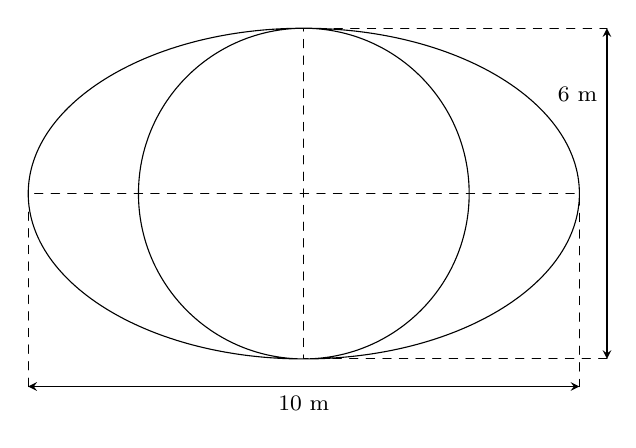
\begin{tikzpicture}[scale=.7, font=\footnotesize, line join=round, line cap=round, >=stealth]
			\def\x{5} 
			\def\y{3} 
			\draw 
			(\x,0) arc (0:-180:{\x} and {\y})
			(\x,0) arc (0:180:{\x} and {\y})
			(0,0) circle (\y)
			;
			\draw[<->] (-5,-3.5)--(5,-3.5)node[pos=.5,below]{$10$ m}
			
			;
			\draw[<->](5.5,-3)--(5.5,3)node[pos=.8,left]{$6$ m};
			\draw[dashed](-5,-3.5)--(-5,0)--(5,0)--(5,-3.5)
			(5.5,-3)--(0,-3)--(0,3)--(5.5,3)
			;
		\end{tikzpicture}
	\end{center}
	\loigiai{
	Theo đề bài ta có $\heva{&2a=10\\&2b=6}\Leftrightarrow\heva{&a=5\\&b=3.}$\\
	Do đường tròn có đường kính bằng độ dài trục nhỏ, suy ra $R=b=3$.\\
	Diện tích phần trồng cỏ là\\
	$\pi ab-\pi R^2=\pi\cdot 5\cdot 3-3^2\cdot\pi=6\pi\approx 18{,}85$ m$^2$.
}
\end{bt}

%Câu 5
\begin{bt}%[0T0B2-2]%[Dự án đề kiểm tra HKII NH22-23- Ngô Quang Anh]%[Ngô Quyền]
	Một nhóm tình nguyện viên gồm $5$ học sinh lớp 10A, $8$ học sinh lớp 10B và $3$ học sinh lớp 10C. Để tham gia một công việc tình nguyện, nhóm có bao nhiêu cách cử ra:
	\begin{enumerate}
		\item $1$ thành viên của nhóm?
		\item $3$ thành viên của nhóm đang học ở ba lớp khác nhau?
		\item Nhóm $3$ bạn có đúng $ 1 $ bạn lớp 10A?
		\item Tính xác suất để chọn ra nhóm $ 4 $ bạn có cả $ 3 $ lớp.
	\end{enumerate}
\loigiai{\begin{enumerate}
		\item Số cách cử ra $1$ thành viên của nhóm là $\mathrm{C}_{16}^1=16$ cách.
		\item Số cách cử ra $3$ thành viên của nhóm học ở ba lớp khác nhau là $\mathrm{C}_{5}^1\cdot\mathrm{C}_{8}^1\cdot\mathrm{C}_{3}^1=120$ cách.
		\item Số cách cử ra $3$ bạn có đúng $1$ bạn lớp 10A là $\mathrm{C}_{5}^1\cdot\mathrm{C}_{11}^2= 55$ cách.
		\item Số phần tử của không gian mẫu là $n\left( \Omega \right)=\mathrm{C}_{16}^4=1820$.\\
		Gọi $A$ là biến cố  \lq\lq chọn ra nhóm $ 4 $ bạn có cả $ 3 $ lớp\rq\rq.\\
		Suy ra $n(A)=\mathrm{C}_{5}^2\cdot\mathrm{C}_{8}^1\cdot\mathrm{C}_{3}^1+\mathrm{C}_{5}^1\cdot\mathrm{C}_{8}^2\cdot\mathrm{C}_{3}^1+\mathrm{C}_{5}^1\cdot\mathrm{C}_{8}^1\cdot\mathrm{C}_{3}^2=780$.\\
		Vậy xác suất cần tìm là $\mathrm{P}(A)=\dfrac{n(A)}{n\left( \Omega \right)}=\dfrac{3}{7}$.
\end{enumerate}}
\end{bt}

%Câu 6
\begin{bt}%[0T9B4-5]%[ID]%[Dự án đề kiểm tra HKII NH22-23- Ngô Quang Anh]%[Ngô Quyền]
	Lập phương trình chính tắc của hypebol có độ dài trục thực bằng $ 6 $ và tiêu cự bằng $ 8 $. 
	\loigiai{
		Vì hypebol có độ dài trục thực bằng $ 6 $ nên $2a=6\Rightarrow a=3$ và
		tiêu cự bằng $ 8 $ nên $c=4$.\\
		Do đó $ b^2=c^2-a^2=4^2-3^2=7$.\\
		Vậy phương trình chính tắc của hypebol là $ \dfrac{x^2}{9}-\dfrac{y^2}{7}=1 $.}
\end{bt}

%Câu 7
\begin{bt}%[0T9B3-3]%[Dự án đề kiểm tra HKII NH22-23- Ngô Quang Anh]%[Ngô Quyền]
	Trong mặt phẳng tọa độ $Oxy$, cho điểm $M(1; 3)$, đường thẳng $d\colon 2x-y+3=0$ và đường tròn $(C)\colon (x-3)^2+(y+2)^2=8$.
	\begin{enumerate}
		\item Viết phương trình đường thẳng $\Delta_1$ qua $M$ và song song với đường thẳng $d$;
		\item Tìm tham số $m$ để $d$ vuông góc với $d^{\prime}\colon 2mx+5y-5=0$;
		\item Viết phương trình tiếp tuyến $\Delta_2$ của đường tròn $(C)$ tại điểm $N(1;-4) \in(C)$.		
	\end{enumerate}
	\loigiai{	\begin{enumerate}
			\item Vì $\Delta_1\parallel d$ nên $\Delta_1\colon 2x-y+d=0$ ($d\ne3$).\\
			$\Delta_1$ qua $M$ nên $2-3+d=0\Rightarrow d=1$ (thỏa).\\
			Vậy $\Delta_1\colon 2x-y+1=0$.
			\item Ta có $d$ và $d^{\prime}$ có véc-tơ pháp tuyến lần lươt là $\vec n_{d}=(2;-1); \vec n_{d'}=(2m;5)$
			 \allowdisplaybreaks
			\begin{eqnarray*}
				d \perp d^{\prime} 
				&\Leftrightarrow& 2m\cdot 2+5\cdot (-1)=0 \\
				&\Leftrightarrow& 4m-5=0 \\
				&\Leftrightarrow& m=\dfrac{5}{4}.
			\end{eqnarray*}
			\item Đường tròn $(C)$ có tâm $I(3;-2)$.\\
			Phương trình tiếp tuyến tại điểm $N(1; -4)$ có dạng:
			\allowdisplaybreaks
			\begin{eqnarray*}
				&&(a-x_0)(x-x_0)+(b-y_0)(y-y_0)=0\\
				&\Leftrightarrow& (3-1)(x-1)+(-2+4)(y+4)=0\\
				&\Leftrightarrow& x+y+3=0.
			\end{eqnarray*}
			Vậy phương trình tiếp tuyến là $x+y+3=0$.		
	\end{enumerate}}
\end{bt}

%Câu 8
\begin{bt}%[0T9K3-5]%[Dự án đề kiểm tra HKII NH22-23- Ngô Quang Anh]%[Ngô Quyền]
	Trong mặt phẳng tọa độ $Oxy$, cho đường thẳng $\Delta\colon x+y+2=0$ và đường tròn $(C)\colon x^2+y^2-4 x-2 y=0$. Gọi $I$ là tâm của $(C)$, $\mathrm{M}$ là điểm thuộc $\Delta$. Qua $\mathrm{M}$ kẻ các tiếp tuyến $MA$ và $MB$ đến $(C)$ ($\mathrm{A}$ và $\mathrm{B}$ là các tiếp điểm). Tìm tọa độ điểm $\mathrm{M}$, biết tứ giác $MAIB$ có diện tích bằng $ 10 $.
	\loigiai{
		\immini{
	Đường tròn $(C)$ có tâm $I(2;1)$, bán kính $R=\sqrt{5}$.\\
	$\mathrm{M}\in \Delta\Rightarrow M(m;-m-2)$.\\
	Do tứ giác $MAIB$ có diện tích bằng $10\Rightarrow IA\cdot AM=10\\\Leftrightarrow AM=2\sqrt{5}$.\\
	Xét tam giác vuông $IAM$ có $IM^2=IA^2+AM^2=25\\\Leftrightarrow m^2+m-6=0\Leftrightarrow  \hoac{&m=2\\&m=-3.}$\\
	Vậy có hai điểm thỏa yêu cầu bài toán là $M(2;-4)$ hoặc $M(-3;1)$.
	}{\begin{tikzpicture}[>=stealth,line join=round,line cap=round,font=\footnotesize,scale=0.9]
		\coordinate[label=above left:$I$] (O) at (0,0);
		\coordinate[label=above:$M$] (M) at (4.11,-1.29);
		\draw (O) circle[radius=2cm]; 
		\coordinate[label=below:$A$] (A) at (0.36,-1.97);
		\coordinate[label=above:$B$] (B) at ($(O)+(45:2cm)$);
		\draw  (M)--(O)--(A)--(B)--(O) ;
		\draw ($(B)!2!90:(O)$)--($(B)!1!-90:(O)$);
		\draw ($(A)!1!90:(O)$)--($(A)!2!-90:(O)$);
		\foreach \diem in {O,A,B,M}\fill (\diem)circle(1pt);
		\draw pic[draw,angle radius=2mm] {right angle = M--A--O};
		\draw pic[draw,angle radius=2mm] {right angle = O--B--M};
	\end{tikzpicture}
	}
	}
\end{bt}

